\documentclass{beamer}
\usepackage{amsfonts,amsmath,oldgerm}
\usetheme{sintef}
\usepackage{listings}
\usepackage{xcolor}
\usepackage{tikz}
\usetikzlibrary{shapes,arrows,positioning,calc,fit,decorations.pathreplacing}

% Color definitions
\definecolor{codegray}{rgb}{0.95,0.95,0.95}
\definecolor{terminalblack}{rgb}{0.1,0.1,0.1}
\definecolor{terminalgreen}{rgb}{0.0,1.0,0.0}
\definecolor{terminalwhite}{rgb}{0.9,0.9,0.9}
\definecolor{terminalred}{rgb}{1.0,0.3,0.3}
\definecolor{terminalyellow}{rgb}{1.0,1.0,0.4}
\definecolor{terminalblue}{rgb}{0.4,0.7,1.0}

% TikZ styles
\tikzset{
    master/.style={draw, rectangle, fill=blue!20, minimum width=3cm, minimum height=1.5cm, text centered, rounded corners},
    worker/.style={draw, rectangle, fill=green!20, minimum width=2.5cm, minimum height=1.2cm, text centered, rounded corners},
    client/.style={draw, rectangle, fill=orange!20, minimum width=2.5cm, minimum height=1.2cm, text centered, rounded corners},
    arrow/.style={->, >=stealth, thick},
    data/.style={draw, rectangle, fill=yellow!10, minimum width=2cm, minimum height=0.8cm, text centered},
    socket/.style={<->, >=stealth, thick, red},
    replica/.style={draw, rectangle, fill=yellow!5, minimum width=2cm, minimum height=0.8cm, text centered, dashed},
    timeline/.style={draw, thick, gray}
}

% Terminal style listing
\lstdefinestyle{terminal}{
    backgroundcolor=\color{terminalblack},
    basicstyle=\small\ttfamily\color{terminalwhite},
    keywordstyle=\color{terminalgreen},
    stringstyle=\color{terminalyellow},
    commentstyle=\color{terminalblue},
    frame=single,
    frameround=tttt,
    framesep=4pt,
    breaklines=true,
    showstringspaces=false,
    columns=fullflexible,
    keepspaces=true,
    xleftmargin=0pt,
    xrightmargin=0pt
}

\usefonttheme[onlymath]{serif}

% \titlebackground*{assets/background}

\newcommand{\hrefcol}[2]{\textcolor{cyan}{\href{#1}{#2}}}

\title{Distributed Array Library}
\subtitle{Concurrent and Distributed Processing}
\course{CC4P1 Concurrent and Distributed Programming}
\author{André Pacheco, Arbues Perez, Sergio Pezo}
\date{July 2025}

\begin{document}
\maketitle

% Index
\begin{frame}
\frametitle{Agenda}
\begin{itemize}
    \item Project Goal
    \item Architecture and Design
    \item Implementation
    \item Communication Protocol
    \item Operation Examples
    \item Replication and Recovery
    \item Fault Tolerance
    \item Demonstration
    \item Conclusions
\end{itemize}
\end{frame}

% Goal
\begin{frame}
\frametitle{Project Goal}
\begin{block}{Develop a distributed library}
    \begin{itemize}
        \item<1-> Distributed arrays: \texttt{DArrayInt} and \texttt{DArrayDouble}
        \item<2-> Concurrent and parallel processing
        \item<3-> Communication via native TCP sockets
        \item<4-> No external frameworks
        \item<5-> Basic fault tolerance
    \end{itemize}
\end{block}

\onslide<6->{
\begin{block}{Implementations}
    \begin{itemize}
        \item Java 8+
        \item Python 3.6+
        \item TypeScript (Client)
    \end{itemize}
\end{block}
}
\end{frame}

% Architecture
\begin{frame}
\frametitle{System Architecture}
\begin{center}
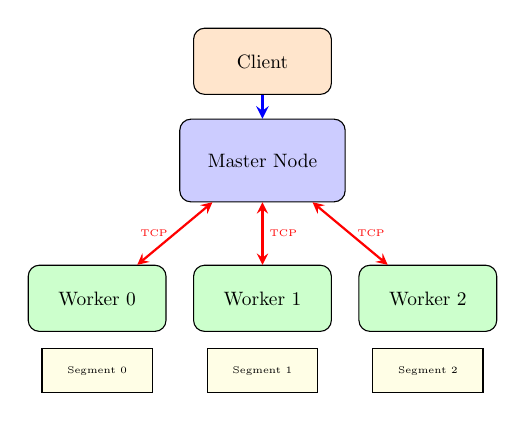
\begin{tikzpicture}[scale=0.7, transform shape]
    % Master node
    \node[master] (master) at (0,2) {Master Node};
    
    % Worker nodes
    \visible<2->{
    \node[worker] (w1) at (-3,-0.5) {Worker 0};
    \node[worker] (w2) at (0,-0.5) {Worker 1};
    \node[worker] (w3) at (3,-0.5) {Worker 2};
    }
    
    % Client
    \visible<3->{
    \node[client] (client) at (0,3.8) {Client};
    }
    
    % Connections
    \visible<2->{
    \draw[socket] (master) -- (w1) node[midway, left] {\tiny TCP};
    \draw[socket] (master) -- (w2) node[midway, right] {\tiny TCP};
    \draw[socket] (master) -- (w3) node[midway, right] {\tiny TCP};
    }
    
    \visible<3->{
    \draw[arrow, blue, line width=1pt] (client) -- (master);
    }
    
    % Data distribution
    \visible<4->{
    \node[data, below=0.3cm of w1] (d1) {\tiny Segment 0};
    \node[data, below=0.3cm of w2] (d2) {\tiny Segment 1};
    \node[data, below=0.3cm of w3] (d3) {\tiny Segment 2};
    }
\end{tikzpicture}
\end{center}

\vspace{-0.5cm}
\visible<5->{
\begin{block}{Features}
    \begin{itemize}
        \item Master-worker architecture
        \item Automatic data distribution
        \item Bidirectional communication
    \end{itemize}
\end{block}
}
\end{frame}

% Implementation - Main classes
\begin{frame}
\frametitle{Implementation - Structure}
\begin{columns}
\column{0.5\textwidth}
\begin{block}{Java}
    \begin{itemize}
        \item<1-> \texttt{MasterNode.java}
        \item<2-> \texttt{WorkerNode.java}
        \item<3-> \texttt{DArrayInt.java}
        \item<3-> \texttt{DArrayDouble.java}
        \item<4-> \texttt{Message.java}
        \item<5-> \texttt{DistributedArrayClient.java}
    \end{itemize}
\end{block}

\column{0.5\textwidth}
\begin{block}{Python / TypeScript}
    \begin{itemize}
        \item<1-> \texttt{master\_node.py}
        \item<2-> \texttt{worker\_node.py}
        \item<3-> \texttt{darray.py}
        \item<4-> \texttt{message.py}
        \item<5-> \texttt{distributed\_array\_client.py}
        \item<6-> \texttt{DistributedArrayClient.ts}
    \end{itemize}
\end{block}
\end{columns}
\end{frame}

% Array Segmentation
\begin{frame}
\frametitle{Array Segmentation}
\begin{center}
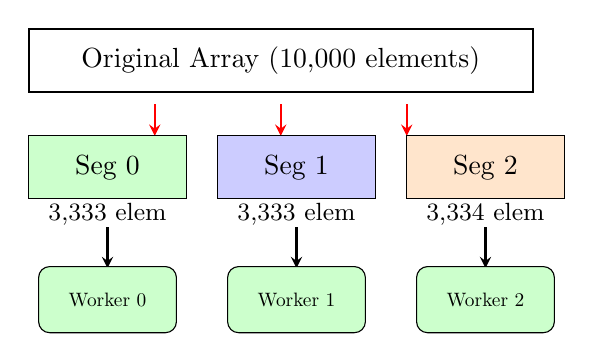
\begin{tikzpicture}[scale=0.8]
    % Original array
    \visible<1->{
    \draw[thick] (0,3.8) rectangle (8,4.8);
    \node at (4,4.3) {Original Array (10,000 elements)};
    }
    
    % Segmentation arrows
    \visible<2->{
    \draw[arrow, red] (2,3.6) -- (2,3.1);
    \draw[arrow, red] (4,3.6) -- (4,3.1);
    \draw[arrow, red] (6,3.6) -- (6,3.1);
    }
    
    % Segments
    \visible<3->{
    \draw[fill=green!20] (0,2.1) rectangle (2.5,3.1);
    \node at (1.25,2.6) {Seg 0};
    \node at (1.25,1.85) {\small 3,333 elem};
    
    \draw[fill=blue!20] (3,2.1) rectangle (5.5,3.1);
    \node at (4.25,2.6) {Seg 1};
    \node at (4.25,1.85) {\small 3,333 elem};
    
    \draw[fill=orange!20] (6,2.1) rectangle (8.5,3.1);
    \node at (7.25,2.6) {Seg 2};
    \node at (7.25,1.85) {\small 3,334 elem};
    }
    
    % Workers
    \visible<4->{
    \draw[arrow] (1.25,1.65) -- (1.25,1);
    \draw[arrow] (4.25,1.65) -- (4.25,1);
    \draw[arrow] (7.25,1.65) -- (7.25,1);
    
    \node[worker, scale=0.7] at (1.25,0.5) {Worker 0};
    \node[worker, scale=0.7] at (4.25,0.5) {Worker 1};
    \node[worker, scale=0.7] at (7.25,0.5) {Worker 2};
    }
\end{tikzpicture}
\end{center}

\vspace{-0.3cm}
\visible<5->{
\begin{block}{Segmentation Algorithm}
    \begin{itemize}
        \item Equal division: $\frac{\text{total}}{\text{workers}}$
        \item Distributed remainder handling
        \item Round-robin assignment
    \end{itemize}
\end{block}
}
\end{frame}

% Communication Protocol
\begin{frame}[fragile]
\frametitle{Communication Protocol}
\begin{block}{JSON Format}
\begin{lstlisting}[basicstyle=\footnotesize\ttfamily]
{
  type: MESSAGE_TYPE,
  from: NODE_ID,
  to: NODE_ID, 
  timestamp: 1234567890,
  data: {},
  status: OK
}
\end{lstlisting}
\end{block}

\vspace{-0.3cm}
\visible<2->{
\begin{block}{Message Types}
    \begin{itemize}
        \small
        \setlength\itemsep{-0.1em}
        \item<2-> \texttt{REGISTER\_WORKER} - Worker registration
        \item<3-> \texttt{DISTRIBUTE\_ARRAY} - Segment distribution
        \item<4-> \texttt{PROCESS\_SEGMENT} - Processing order
        \item<5-> \texttt{HEARTBEAT} - Health check
        \item<6-> \texttt{REPLICATE\_DATA} - Segment replication
        \item<7-> \texttt{RECOVER\_DATA} - Failure recovery
    \end{itemize}
\end{block}
}
\end{frame}

% Parallel Processing
\begin{frame}
\frametitle{Parallel Processing}
\begin{center}
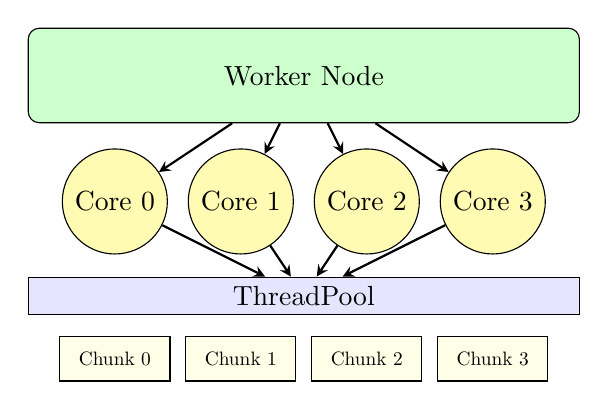
\begin{tikzpicture}[scale=0.8]
    % Worker node
    \node[worker, minimum width=7cm] (worker) at (0,4) {Worker Node};
    
    % CPU cores
    \visible<2->{
    \node[draw, circle, fill=yellow!30] (c1) at (-3,2) {Core 0};
    \node[draw, circle, fill=yellow!30] (c2) at (-1,2) {Core 1};
    \node[draw, circle, fill=yellow!30] (c3) at (1,2) {Core 2};
    \node[draw, circle, fill=yellow!30] (c4) at (3,2) {Core 3};
    
    \draw[arrow] (worker) -- (c1);
    \draw[arrow] (worker) -- (c2);
    \draw[arrow] (worker) -- (c3);
    \draw[arrow] (worker) -- (c4);
    }
    
    % Thread pool
    \visible<3->{
    \node[draw, rectangle, fill=blue!10, minimum width=7cm] (pool) at (0,0.5) {ThreadPool};
    \draw[arrow] (c1) -- (pool);
    \draw[arrow] (c2) -- (pool);
    \draw[arrow] (c3) -- (pool);
    \draw[arrow] (c4) -- (pool);
    }
    
    % Data chunks
    \visible<4->{
    \node[data, scale=0.7] at (-3,-0.5) {Chunk 0};
    \node[data, scale=0.7] at (-1,-0.5) {Chunk 1};
    \node[data, scale=0.7] at (1,-0.5) {Chunk 2};
    \node[data, scale=0.7] at (3,-0.5) {Chunk 3};
    }
\end{tikzpicture}
\end{center}

\vspace{-0.3cm}
\visible<5->{
\begin{block}{Strategy}
    \begin{itemize}
        \small
        \setlength\itemsep{-0.1em}
        \item Automatic core detection: \texttt{Runtime.availableProcessors()}
        \item Division of the segment into chunks
        \item Concurrent processing with ThreadPool
        \item Synchronization using \texttt{Future<T>}
    \end{itemize}
\end{block}
}
\end{frame}

% Example 1 - Mathematical Operations
\begin{frame}
\frametitle{Example 1: Mathematical Operations}
\begin{block}{Formula}
$$\text{result} = \frac{(\sin(x) + \cos(x))^2}{\sqrt{|x|} + 1}$$
\end{block}

\visible<2->{
\begin{block}{Java Implementation}
    \begin{itemize}
        \item Parallel processing with ThreadPool
        \item Division of the segment into chunks
        \item Each thread processes its chunk independently
    \end{itemize}
\end{block}
}

\visible<3->{
\begin{block}{Python Implementation}
    \begin{itemize}
        \item Use of ThreadPoolExecutor
        \item NumPy for vectorized operations
        \item Concurrent processing by chunks
    \end{itemize}
\end{block}
}
\end{frame}

% Example 2 - Conditional Evaluation
\begin{frame}
\frametitle{Example 2: Conditional Evaluation}
\begin{block}{Condition}
If $x \bmod 3 = 0$ or $500 \leq x \leq 1000$:
$$\text{result} = (x \cdot \log(x)) \bmod 7$$
\end{block}

\visible<2->{
\begin{block}{Processing}
    \begin{itemize}
        \item Conditional evaluation for each element
        \item Application of logarithmic transformation
        \item Preservation of values that do not meet the condition
    \end{itemize}
\end{block}
}

\visible<3->{
\begin{block}{Resilience}
    \begin{itemize}
        \item Exception handling per thread
        \item Continuation in case of partial failures
        \item Consolidation of valid results
    \end{itemize}
\end{block}
}
\end{frame}

% Replication and Recovery
\begin{frame}
\frametitle{Data Replication}
\begin{center}
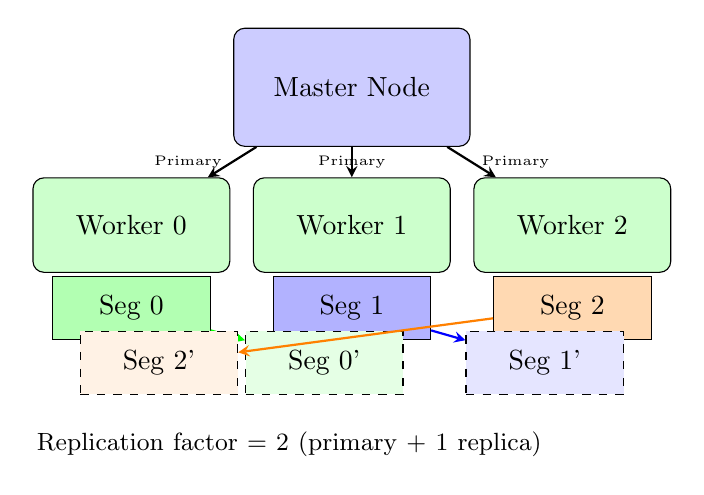
\begin{tikzpicture}[scale=0.7]
    % Master
    \node[master] (master) at (0,3.5) {Master Node};
    
    % Workers
    \node[worker] (w1) at (-4,1) {Worker 0};
    \node[worker] (w2) at (0,1) {Worker 1};
    \node[worker] (w3) at (4,1) {Worker 2};
    
    % Array segments
    \visible<2->{
    \node[data, fill=green!30] (s0) at (-4,-0.5) {Seg 0};
    \node[data, fill=blue!30] (s1) at (0,-0.5) {Seg 1};
    \node[data, fill=orange!30] (s2) at (4,-0.5) {Seg 2};
    }
    
    % Primary assignments
    \visible<3->{
    \draw[arrow, thick] (master) -- (w1) node[midway, left] {\tiny Primary};
    \draw[arrow, thick] (master) -- (w2) node[midway] {\tiny Primary};
    \draw[arrow, thick] (master) -- (w3) node[midway, right] {\tiny Primary};
    }
    
    % Replicas
    \visible<4->{
    % Replica of Seg 0 on Worker 1
    \node[replica, fill=green!10] (s0r) at (-0.5,-1.5) {Seg 0'};
    \draw[arrow, green] (s0) -- (s0r);
    
    % Replica of Seg 1 on Worker 2
    \node[replica, fill=blue!10] (s1r) at (3.5,-1.5) {Seg 1'};
    \draw[arrow, blue] (s1) -- (s1r);
    
    % Replica of Seg 2 on Worker 0
    \node[replica, fill=orange!10] (s2r) at (-3.5,-1.5) {Seg 2'};
    \draw[arrow, orange] (s2) -- (s2r);
    }
    
    \visible<5->{
    \node[below=3.5cm of master, text width=8cm] {\small Replication factor = 2 (primary + 1 replica)};
    }
\end{tikzpicture}
\end{center}
\end{frame}

% Recovery Mechanism
\begin{frame}
\frametitle{Recovery Mechanism}
\begin{columns}
\column{0.5\textwidth}
\begin{block}{Failure Detection}
    \begin{enumerate}
        \item<1-> Heartbeat timeout (10s)
        \item<2-> Worker marked as down
        \item<3-> Activate recovery process
    \end{enumerate}
\end{block}

\visible<4->{
\begin{block}{Replica Promotion}
    \begin{enumerate}
        \item Identify affected segments
        \item Promote replicas to primary
        \item Update segment mappings
    \end{enumerate}
\end{block}
}

\column{0.5\textwidth}
\visible<5->{
\begin{block}{New Replica Creation}
    \begin{enumerate}
        \item Select available workers
        \item Replicate data from primary
        \item Maintain replication factor
    \end{enumerate}
\end{block}
}

\visible<6->{
\begin{block}{Redistribution}
    \begin{enumerate}
        \item Balance load among workers
        \item Avoid node overload
        \item Optimize resource usage
    \end{itemize}
\end{block}
}
\end{columns}
\end{frame}

% Example 3 - Failure Simulation
\begin{frame}
\frametitle{Example 3: Fault Recovery}
\begin{center}
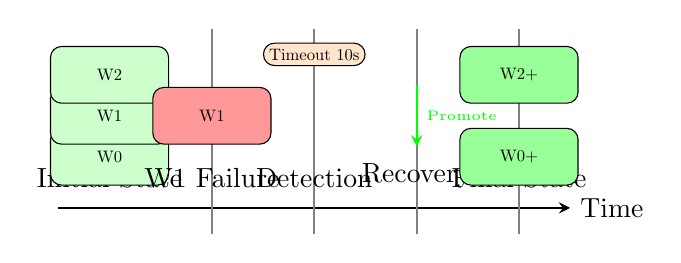
\begin{tikzpicture}[scale=0.65]
    % Timeline
    \draw[arrow] (0,0) -- (10,0) node[right] {Time};
    
    % States
    \visible<1->{
    \node[above] at (1,0.2) {Initial State};
    \node[worker, scale=0.6] at (1,1) {W0};
    \node[worker, scale=0.6] at (1,1.8) {W1};
    \node[worker, scale=0.6] at (1,2.6) {W2};
    }
    
    \visible<2->{
    \draw[timeline] (3,-0.5) -- (3,3.5);
    \node[above] at (3,0.2) {W1 Failure};
    \node[worker, scale=0.6, fill=red!40] at (3,1.8) {W1};
    }
    
    \visible<3->{
    \draw[timeline] (5,-0.5) -- (5,3.5);
    \node[above] at (5,0.2) {Detection};
    \node[draw, fill=orange!20, rounded corners, scale=0.6] at (5,3) {Timeout 10s};
    }
    
    \visible<4->{
    \draw[timeline] (7,-0.5) -- (7,3.5);
    \node[above] at (7,0.2) {Recovery};
    \draw[arrow, green] (7,2.4) -- (7,1.2) node[midway, right] {\tiny Promote};
    }
    
    \visible<5->{
    \draw[timeline] (9,-0.5) -- (9,3.5);
    \node[above] at (9,0.2) {Final State};
    \node[worker, scale=0.6, fill=green!40] at (9,1) {W0+};
    \node[worker, scale=0.6, fill=green!40] at (9,2.6) {W2+};
    }
\end{tikzpicture}
\end{center}

\vspace{0.5cm}
\visible<6->{
\begin{block}{Automatic Process}
    \begin{itemize}
        \item No data loss
        \item Service continuity
        \item Transparent to the client
    \end{itemize}
\end{block}
}
\end{frame}

% Terminal output for recovery demo
\begin{frame}[fragile]
\frametitle{Demonstration - Automatic Recovery}
\begin{lstlisting}[style=terminal]
$ ./test-recovery.sh
=== Distributed Array Recovery Test ===
Starting Master node on port 5000
Starting Worker-1
Starting Worker-2
Starting Worker-3

=== Creating distributed array ===
Create array response: {status:created,arrayId:myArray}
INFO: Replicated segment 0 to worker-2
INFO: Replicated segment 100 to worker-3
INFO: Replicated segment 200 to worker-1

=== Simulating Worker-2 failure ===
Worker-2 has been terminated!
WARNING: Worker worker-2 failed health check
ERROR: Handling failure of worker: worker-2

=== Recovery in progress ===
INFO: Promoted replica worker-1 for segment 0 of array myArray
INFO: Created new replica on worker-3 for segment 0
INFO: Recovery completed successfully

=== Testing array operations after recovery ===
Apply operation response: {status:processing}
Operations completed successfully after recovery!
\end{lstlisting}
\end{frame}

% Fault Tolerance
\begin{frame}
\frametitle{Fault Tolerance}
\begin{center}
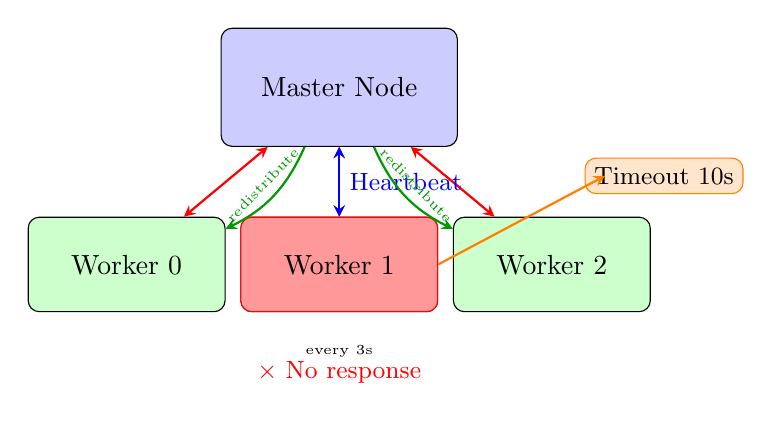
\begin{tikzpicture}[scale=0.75]
    % Master node
    \node[master] (master) at (0,3) {Master Node};
    
    % Workers
    \visible<1->{
    \node[worker] (w1) at (-3.6,0) {Worker 0};
    \node[worker] (w2) at (0,0) {Worker 1};
    \node[worker] (w3) at (3.6,0) {Worker 2};
    
    % Connections
    \draw[socket] (master) -- (w1);
    \draw[socket] (master) -- (w2);
    \draw[socket] (master) -- (w3);
    }
    
    % Heartbeat signals
    \visible<2->{
    \draw[arrow, blue, thick, <->] (master.south) -- (w2.north) node[midway, right] {\small Heartbeat};
    \node[below=0.3cm of w2] {\tiny every 3s};
    }
    
    % Worker failure
    \visible<3->{
    \node[worker, fill=red!40, draw=red] (w2fail) at (0,0) {Worker 1};
    \node[below=0.5cm of w2fail, red] {\small $\times$ No response};
    }
    
    % Detection
    \visible<4->{
    \node[draw=orange, fill=orange!20, rounded corners] at (5.5,1.5) {\small Timeout 10s};
    \draw[arrow, orange, thick] (w2fail.east) -- (4.5,1.5);
    }
    
    % Redistribution
    \visible<5->{
    \draw[arrow, green!60!black, thick, bend left=20] (master) to node[above, sloped] {\tiny redistribute} (w1);
    \draw[arrow, green!60!black, thick, bend right=20] (master) to node[above, sloped] {\tiny redistribute} (w3);
    }
\end{tikzpicture}
\end{center}

\visible<6->{
\begin{block}{Fault Tolerance System}
    \begin{itemize}
        \item Heartbeat: check every 3 seconds
        \item Detection: 10-second timeout
        \item Replication: factor 2 (primary + replica)
        \item Recovery: automatic promotion of replicas
        \item Redistribution: creation of new replicas
    \end{itemize}
\end{block}
}
\end{frame}

% Demonstration - Terminal Output
\begin{frame}[fragile]
\frametitle{Demonstration - Cluster Start}
\begin{lstlisting}[style=terminal]
$ ./start-java-cluster.sh
Starting Java distributed array cluster...
Starting master node on port 5000...
Master node PID: 12345
Starting worker-0...
Worker-0 PID: 12346
Starting worker-1...
Worker-1 PID: 12347
Starting worker-2...
Worker-2 PID: 12348

Java cluster started successfully!
Master node running on port 5000
3 worker nodes connected
\end{lstlisting}
\end{frame}

% TypeScript Client
\begin{frame}[fragile]
\frametitle{TypeScript Client}
\begin{block}{Features}
    \begin{itemize}
        \item<1-> Full client in TypeScript/Node.js
        \item<2-> Compatible with Java and Python clusters
        \item<3-> Identical CLI interface
        \item<4-> Asynchronous communication with Promises
        \item<5-> Strong typing with interfaces
    \end{itemize}
\end{block}

\visible<6->{
\begin{block}{Usage Example}
\footnotesize
\texttt{\$ npm start -- localhost 5000}\\
\texttt{Connected to master at localhost:5000}\\
\texttt{Enter commands (type help for usage, exit to quit):}\\
\texttt{> create-double ts-array 5000}\\
\texttt{Create array response: \{status:created\}}\\
\texttt{> apply ts-array example1}\\
\texttt{Apply operation response: \{status:processing\}}
\end{block}
}
\end{frame}

% Interactive Client
\begin{frame}[fragile]
\frametitle{Demonstration - Interactive Client}
\begin{lstlisting}[style=terminal]
$ java -cp out:lib/* client.DistributedArrayClient localhost 5000
Connected to master at localhost:5000
Enter commands (type help for usage, exit to quit):
> create-double math-array 10000
Create array response: {type:OPERATION_COMPLETE,
  data:{arrayId:math-array,status:created}}

> apply math-array example1
Apply operation response: {type:OPERATION_COMPLETE,
  data:{status:processing}}

> get math-array
Get result response: {type:OPERATION_COMPLETE,
  data:{status:complete,result:Operation completed}}
\end{lstlisting}
\end{frame}

% System Logs
\begin{frame}[fragile]
\frametitle{System Logs}
\begin{lstlisting}[style=terminal]
master.log
INFO: Master node started on port 5000
INFO: Worker registered: worker-0 from 127.0.0.1
INFO: Worker registered: worker-1 from 127.0.0.1
INFO: Worker registered: worker-2 from 127.0.0.1
INFO: Received array creation request: math-array (10000 elements)
INFO: Array segmented: 3 segments distributed
INFO: Processing operation: example1 on math-array

worker-0.log
INFO: Registered with master node
INFO: Received double array segment: math-array with 3333 elements
INFO: Processing Example 1 using 4 threads
INFO: Completed Example 1 processing for math-array
INFO: Sent result to master
\end{lstlisting}
\end{frame}

% Performance
\begin{frame}
\frametitle{Performance and Scalability}
\begin{columns}
\column{0.5\textwidth}
\begin{block}{Parallelization}
    \begin{itemize}
        \item<1-> Use of all cores
        \item<2-> Efficient ThreadPool
        \item<3-> Automatic work division
    \end{itemize}
\end{block}

\visible<4->{
\begin{block}{Distribution}
    \begin{itemize}
        \item Equal segmentation
        \item Asynchronous communication
        \item Independent processing
    \end{itemize}
\end{block}
}

\column{0.5\textwidth}
\visible<5->{
\begin{block}{Metrics (10,000 elements)}
    \begin{itemize}
        \item 1 worker: 250ms
        \item 2 workers: 140ms
        \item 3 workers: 95ms
        \item 4 workers: 75ms
    \end{itemize}
\end{block}
}
\end{columns}

\visible<6->{
\begin{center}
\begin{tikzpicture}[scale=0.6]
    \draw[->] (0,0) -- (5,0) node[right] {Workers};
    \draw[->] (0,0) -- (0,4) node[above] {Time (ms)};
    
    \draw[thick, blue] (1,3.5) -- (2,2) -- (3,1.3) -- (4,1);
    
    \foreach \x in {1,2,3,4} {
        \draw (\x,0.1) -- (\x,-0.1) node[below] {\x};
    }
\end{tikzpicture}
\end{center}
}
\end{frame}

% Conclusions
\begin{frame}
\frametitle{Conclusions}
\begin{block}{Achievements}
    \begin{itemize}
        \item<1-> Functional library in Java, Python, and TypeScript
        \item<2-> Truly distributed processing
        \item<3-> Effective parallelization per node
        \item<4-> Complete replication and recovery system
        \item<5-> No external framework dependencies
        \item<6-> Interoperability between languages
    \end{itemize}
\end{block}

\visible<6->{
\begin{block}{Applications}
    \begin{itemize}
        \item Large dataset processing
        \item Distributed scientific calculations
        \item Parallel data analysis
    \end{itemize}
\end{block}
}

\visible<7->{
\begin{block}{Advanced Implemented Features}
    \begin{itemize}
        \item Automatic segment replication
        \item Transparent fault recovery
        \item Replication factor maintenance
        \item Dynamic data redistribution
    \end{itemize}
\end{block}
}
\end{frame}

% Questions
\begin{frame}
\frametitle{Questions}
\begin{center}
\Large{Thank you for your attention}

\vspace{1cm}

\normalsize
GitHub: \url{https://github.com/A-PachecoT/distributed-array-lib}

\vspace{0.5cm}

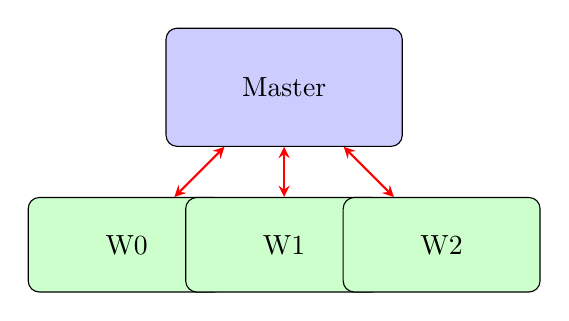
\begin{tikzpicture}
    \node[master] (m) at (0,0) {Master};
    \node[worker] (w1) at (-2,-2) {W0};
    \node[worker] (w2) at (0,-2) {W1};
    \node[worker] (w3) at (2,-2) {W2};
    
    \draw[socket] (m) -- (w1);
    \draw[socket] (m) -- (w2);
    \draw[socket] (m) -- (w3);
\end{tikzpicture}
\end{center}
\end{frame}

\end{document}